\section{Zielsetzung}
\label{sec:Zielsetzung}
Das Ziel des Versuches ist das Bestimmen verschiedener ohmscher Widerstände, Kapazitäten und Induktivitäten durch ausgewählte Brückenschaltungen. Außerdem werden 
durch den Versuch das Verständnis der Kirchhoffschen Gesetze vertieft und verschiedene Brückenschaltungen vorgestellt.  

\section{Theorie}
\label{sec:Theorie}
    \subsection{Funktonsprinzip einer Brückenschaltung}
    Die Funktionsweise einer Brückenschaltung beruht auf zwei Kirchhoffschen Gesetzen. Die sogenannte Knotenregel besagt, dass an einem Knotenpunkt die Summe der 
    zufließenden Ströme der Summe der abfließenden Ströme entsprechen muss. Zufließende Ströme haben ein positives Vorzeichen und abfließende Ströme haben ein 
    negatives Vorzeichen. Dann gilt 
    \begin{equation}
        \label{eqn:Knotenregel}
        \sum_k {I_k} = 0 \,.
    \end{equation}
    $I_k$ sind dabei die einzelnen zufließende oder abfließende Ströme. 
    Die sogenannte Maschenregel beschreibt, dass die Summe aller treibenden, elektrischen Spannungen der Summe der abfallenden Spannungen innerhalb einer beliebigen, geschlossenen 
    Masche eines Stromkreises entspricht. Dabei haben die abfallenden Spannung ein negatives Vorzeichen und die treibenden Spannungen ein positives Vorzeichen. 
    Dann gilt
    \begin{equation}
        \label{eqn:Maschenregel}
        \sum_k {U_k} = 0 
    \end{equation}
    innerhalb einer Masche. $U_k$ sind dabei die in der Masche treibenden oder abfallenden Spannungen. 
    Diese beiden Regel können verwendet werden, um Schaltpläne zu erstellen, die es ermöglichen die Kenngrößen unbekannter Bauteile zu bestimmen. Eine 
    solche prinzipielle Brückenschaltung ist in Abbildung (\ref{pic:prinzipielle_Brückenschaltung}) zu sehen. $R$ bezeichnet ohmsche Widerstände.
    \section{Durchführung}
\label{sec:Durchführung}
\begin{figure}[H]
    \centering
    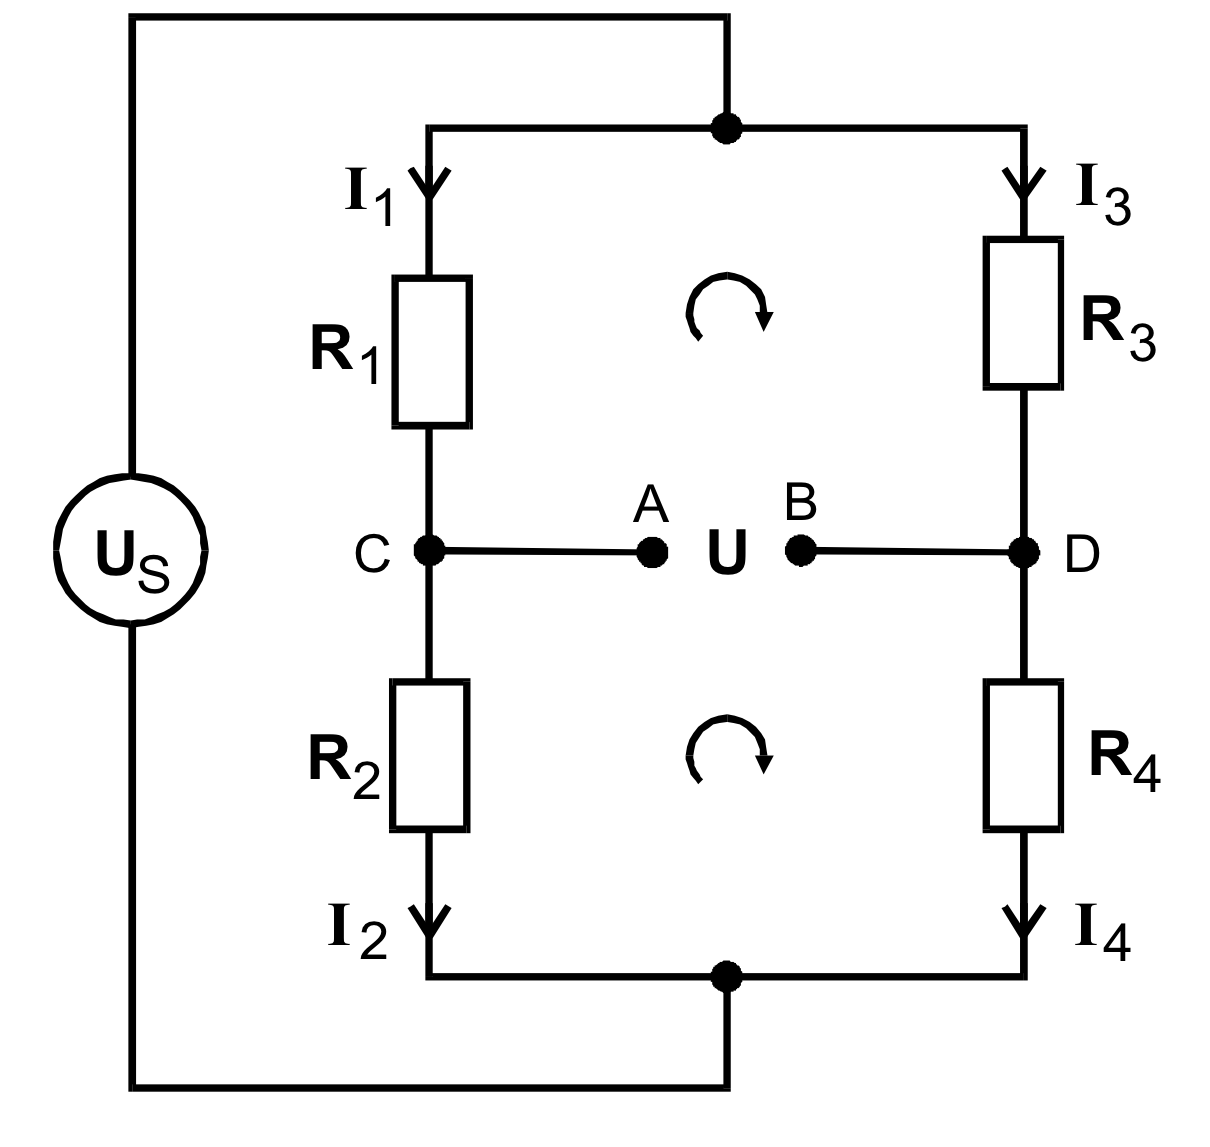
\includegraphics[width=0.4\linewidth]{prinzipielle_Schaltung.png}
    \caption{Schaltplan einer prinzipiellen Brückenschaltung}
    \label{pic:prinzipielle_Brückenschaltung}
\end{figure}
Die unbekannte Kenngröße wird durch die sogenannte Nullmethode bestimmt. Bei dieser wird $R_2$ variiert bis zwischen Punkt A und Punkt B keine Spannung mehr zu
messen ist. 
\subsection{Wheatstonesche Brücke}
In der Whaéatstoneschen Brückenschaltung werden jeweils zwei in Reihe geschaltete ohmsche WIderstände parallel zueinander gechaltet, wie im Schaltplan in Abbildung 
(\ref{}) zu sehen. 
Die Wheatstonesche Brückeschaltung wird verwendet, um einen unbekannten ohmschen Widerstand $R_x$ zu bestimmen. Dies erfolgt durch die Formel 
\begin{equation}
    \label{eqn:Wheatstone_R}
    R_x = R_2 \cdot \frac{R_3}{R_4} \,.
\end{equation}
\subsection{Kapazitätsmessbrücke}
\subsection{Induktivitätsmessbrücke}
\subsection{Maxwell-Brücke}
\subsection{Wien-Robinson-Brücke}
\subsection{Kirrfaktor}



